\chapter{Your 90-Day Automation Action Plan}

%! suppress = LineBreak
\begin{warningblock}
    This is an Early Release. You're getting the raw and unedited content as I write. I'm doing this, so you can take advantage of the content
    before the official release, AND you can share critical feedback (plus, I include you in the credits of the official release)
    To get notified when I add new section(s), \href{https://discord.gg/X2USgYTB}{join the Business Automators discord community}
\end{warningblock}
\begin{importantblock}
    If you found a problem, \href{https://discord.gg/X2USgYTB}{drop a comment in the discord community} or  \href{mailto:dele@protomated.com}{email dele@protomated.com}.
\end{importantblock}


%
%

\section{Introduction}

Welcome to your 90-day automation journey! This chapter will guide you through a comprehensive action plan to transform your IT consulting practice through automation. We'll break down the next three months into manageable bi-weekly segments, each building upon the last to help you progressively enhance your automation skills and deliver tangible results for your clients.

Throughout this journey, we'll focus on leveraging the key tools we've explored in this book: n8n for workflow automation, NoCoDB for database management, and BudiBase for creating custom applications. We'll also incorporate other complementary tools as needed to create a well-rounded automation toolkit.

Remember, the goal isn't just to learn these tools in isolation, but to apply them to real-world problems and create meaningful automations for your clients. By the end of these 90 days, you'll have completed several automation projects, integrated multiple systems, and significantly enhanced your capabilities as an IT consultant.

Let's start by outlining our key objectives for this 90-day plan:

\begin{itemize}
    \item Complete at least 6 automation projects (one every two weeks)
    \item Integrate at least 3 different systems or tools
    \item Achieve measurable improvements in efficiency (time saved) and client satisfaction
    \item Overcome common technical challenges in implementation and data integration
    \item Build a portfolio of successful automations to showcase to potential clients
\end{itemize}

To keep track of your progress, I've included a weekly progress tracker as an addendum to this chapter. Use this to monitor your achievements, note challenges, and stay motivated throughout the journey.

Importantly, you're not alone on this journey. We encourage you to regularly check in with the Business Automators community at \url{https://discord.gg/X2USgYTB}. Share your successes, ask for help with challenges, and learn from others who are on the same path. Remember, every small win is worth celebrating, and every obstacle overcome is a valuable lesson learned.

Now, let's dive into your bi-weekly action plan!

\section{Weeks 1-2: Foundation and First Automation}

\subsection{Objectives}
\begin{itemize}
    \item Set up your automation environment
    \item Complete your first basic automation project
    \item Establish baseline metrics for time spent on manual tasks
\end{itemize}

\subsection{Action Steps}

\subsubsection{Step 1: Environment Setup}
Begin by setting up your automation toolkit:

\begin{itemize}
    \item Install and configure n8n locally or set up a cloud instance
    \item Set up a NoCoDB instance for data management
    \item Install BudiBase for creating custom applications
\end{itemize}

% TODO @screenshot: Show the setup screens for n8n, NoCoDB, and BudiBase side by side

\subsubsection{Step 2: Identify Your First Automation Project}
Choose a simple, high-impact task to automate. Consider starting with one of these:

\begin{itemize}
    \item Automate email responses for common client inquiries
    \item Create a simple task management system
    \item Set up automated reporting for a client project
\end{itemize}

\subsubsection{Step 3: Implement Your First Automation}
Use n8n to create a workflow for your chosen task. Here's a basic example of an automated email response system:

% TODO @illustrate: Diagram of a simple n8n workflow for email automation (see PDF for caption, ``A simple n8n workflow for email automation'')

\begin{figure}[H]
    \centering
    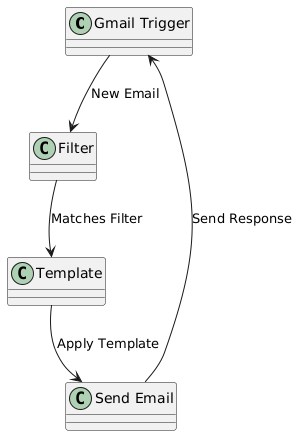
\includegraphics{figures/09-gmail-flow-example}
    \caption{A simple n8n workflow for email automation}
    \label{fig:09-gmail-flow-example}
\end{figure}



\subsubsection{Step 4: Measure and Record Baseline Metrics}
Before fully implementing your automation, measure how long the task takes manually. Record this in your progress tracker. This will be crucial for demonstrating the value of your automation efforts later.

\subsection{Common Challenges and Solutions}
\begin{itemize}
    \item Challenge: Difficulty in setting up the tools
    \item Solution: Refer to the official documentation and don't hesitate to ask for help in the Business Automators community

    \item Challenge: Choosing the right first project
    \item Solution: Start small. It's better to complete a simple automation successfully than to get stuck on a complex one
\end{itemize}

\subsection{Check-In and Reflection}
At the end of week 2, reflect on your progress:

\begin{itemize}
    \item Did you successfully set up your environment?
    \item Have you completed your first automation project?
    \item What challenges did you face, and how did you overcome them?
    \item Share your progress in the Business Automators Discord community
\end{itemize}

\section{Weeks 3-4: Expanding Your Toolkit}

\subsection{Objectives}
\begin{itemize}
    \item Integrate NoCoDB into your automation workflows
    \item Complete a more complex automation project
    \item Start measuring time saved through automation
\end{itemize}

\subsection{Action Steps}

\subsubsection{Step 1: NoCoDB Integration}
Enhance your existing automation or create a new one that incorporates NoCoDB:

\begin{itemize}
    \item Set up a database in NoCoDB to store client information or project data
    \item Use n8n to create a workflow that reads from or writes to your NoCoDB database
\end{itemize}

Here's an example of how you might integrate NoCoDB into an n8n workflow:

% TODO @illustrate: Diagram showing n8n workflow with NoCoDB integration (see PDF for caption: `n8n workflow with NoCoDB integration'')
\begin{figure}[H]
    \centering
    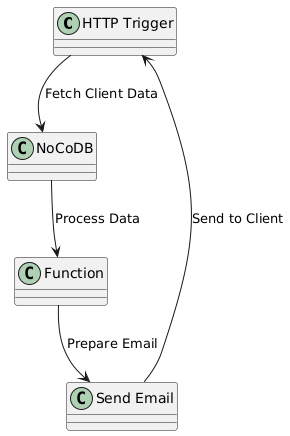
\includegraphics[width=0.5\textwidth]{figures/09-n8n-with-budibase}
    \caption{n8n workflow with NoCoDB integration}
    \label{fig:n8n-with-budibase}
\end{figure}


\subsubsection{Step 2: Implement a More Complex Automation}
Build upon your skills to create a more sophisticated automation. Some ideas:

\begin{itemize}
    \item Automate client onboarding process
    \item Create a system for automated time tracking and invoicing
    \item Set up a workflow for collecting and analyzing client feedback
\end{itemize}

\subsubsection{Step 3: Measure Time Savings}
Start tracking the time saved by your automations:

\begin{itemize}
    \item Compare the time taken for manual processes vs. automated ones
    \item Record these metrics in your progress tracker
    \item Calculate the potential time savings if applied across all your clients
\end{itemize}

\subsection{Common Challenges and Solutions}
\begin{itemize}
    \item Challenge: Difficulty in data integration between systems
    \item Solution: Ensure you understand the data structures of both systems. Use n8n's data mapping features to correctly align fields

    \item Challenge: Automation not working as expected
    \item Solution: Use n8n's built-in testing features to debug your workflow step by step. Don't hesitate to break down complex workflows into smaller, manageable parts
\end{itemize}

\subsection{Check-In and Reflection}
At the end of week 4, assess your progress:

\begin{itemize}
    \item Have you successfully integrated NoCoDB into your workflow?
    \item Did you complete a more complex automation project?
    \item Can you quantify the time savings from your automations?
    \item Share your achievements and any interesting insights in the Business Automators Discord community
\end{itemize}

\section{Weeks 5-6: Introducing BudiBase and Enhancing Client Interaction}

\subsection{Objectives}
\begin{itemize}
    \item Create your first BudiBase application
    \item Integrate BudiBase with your existing automations
    \item Implement a client-facing dashboard or tool
\end{itemize}

\subsection{Action Steps}

\subsubsection{Step 1: BudiBase Basics}
Start by creating a simple application in BudiBase:

\begin{itemize}
    \item Design a basic client management or project tracking app
    \item Connect it to your NoCoDB database for data storage
    \item Familiarize yourself with BudiBase's UI components and logic
\end{itemize}

% TODO @screenshot: Show a simple BudiBase application interface

\subsubsection{Step 2: Integrate BudiBase with n8n}
Enhance your automation by connecting BudiBase and n8n:

\begin{itemize}
    \item Use n8n to trigger actions in your BudiBase app
    \item Create workflows that respond to events in your BudiBase application
\end{itemize}

Here's an example of how you might integrate BudiBase into your automation ecosystem:

% TODO @illustrate: Diagram showing integration between n8n, NoCoDB, and BudiBase

\begin{figure}
    \centering
    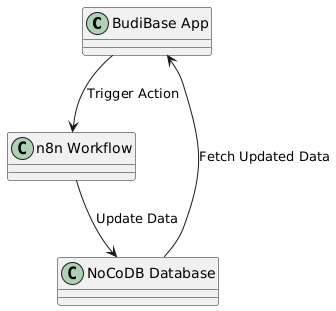
\includegraphics[width=0.5\textwidth]{figures/09-n8n-budibase-nocodb}
    \caption{Integration between n8n, NoCoDB, and BudiBase}
    \label{fig:n8n-budibase-nocodb-integration}
\end{figure}

\subsubsection{Step 3: Create a Client-Facing Tool}
Develop a tool or dashboard that provides value directly to your clients:

\begin{itemize}
    \item Design a project status dashboard
    \item Create a self-service portal for common client requests
    \item Implement a reporting tool that automatically generates and sends reports to clients
\end{itemize}

\subsection{Common Challenges and Solutions}
\begin{itemize}
    \item Challenge: Designing intuitive user interfaces in BudiBase
    \item Solution: Start with BudiBase templates and customize them. Gather feedback from team members or trusted clients to improve usability

    \item Challenge: Ensuring data consistency across different tools
    \item Solution: Implement data validation in your n8n workflows. Use NoCoDB's data integrity features to maintain consistency
\end{itemize}

\subsection{Check-In and Reflection}
As you reach the halfway point of your 90-day journey, take stock of your progress:

\begin{itemize}
    \item Have you created a functional BudiBase application?
    \item Did you successfully integrate BudiBase with your existing automations?
    \item How has client interaction improved with your new tools?
    \item Share a screenshot or description of your client-facing tool in the Business Automators Discord community
\end{itemize}

\section{Weeks 7-8: Advanced Automation and Integration}

\subsection{Objectives}
\begin{itemize}
    \item Implement more advanced n8n features
    \item Integrate with external APIs or services
    \item Create a complex, multi-step automation workflow
\end{itemize}

\subsection{Action Steps}

\subsubsection{Step 1: Explore Advanced n8n Features}
Dive deeper into n8n's capabilities:

\begin{itemize}
    \item Experiment with error handling and retry mechanisms
    \item Use n8n's looping features for batch processing
    \item Implement conditional workflows for more complex logic
\end{itemize}

\subsubsection{Step 2: External API Integration}
Expand your automation capabilities by integrating with external services:

\begin{itemize}
    \item Connect to a CRM system like Salesforce or HubSpot
    \item Integrate with project management tools like Jira,  Trello or Nifty PM
    \item Implement automation with cloud storage services like Google Drive or Dropbox
\end{itemize}

Here's an example of a more complex workflow integrating multiple services:

% TODO @illustrate: Diagram of a complex n8n workflow with multiple integrations (See PDF caption ``A complex n8n workflow with multiple integrations'')

\begin{figure}
    \centering
    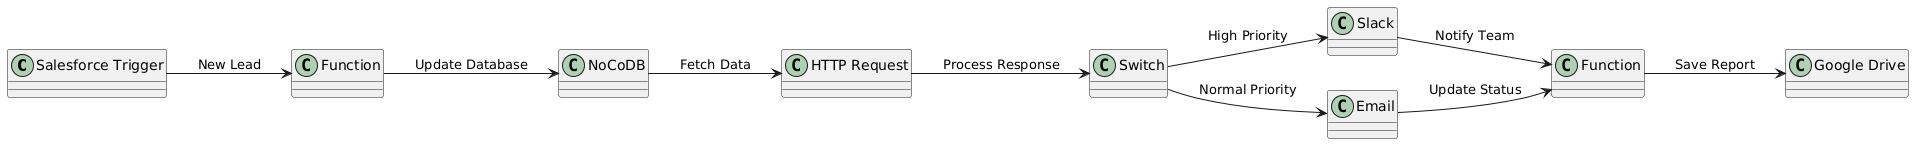
\includegraphics[width=0.5\textwidth]{figures/09-complex-n8n-workflow}
    \caption{A complex n8n workflow with multiple integrations}
    \label{fig:complex-n8n-workflow}
\end{figure}

\subsubsection{Step 3: Implement a Complex Workflow}
Put everything together to create a sophisticated automation:

\begin{itemize}
    \item Automate a complete business process (e.g., from lead generation to project completion)
    \item Implement error handling, notifications, and fallback mechanisms
    \item Ensure the workflow integrates with your BudiBase application and NoCoDB database
\end{itemize}

\subsection{Common Challenges and Solutions}
\begin{itemize}
    \item Challenge: Managing complex workflows with multiple steps and conditions
    \item Solution: Use n8n's organizational features like notes and groups. Consider breaking very complex workflows into multiple, interconnected workflows

    \item Challenge: Dealing with API rate limits and timeouts
    \item Solution: Implement retry mechanisms and use n8n's queueing features. Consider using webhook nodes for real-time updates where possible
\end{itemize}

\subsection{Check-In and Reflection}
As you complete this advanced section, reflect on your growth:

\begin{itemize}
    \item What new n8n features have you mastered?
    \item How have external integrations expanded your automation capabilities?
    \item What was the most challenging part of creating a complex workflow, and how did you overcome it?
    \item Share insights about your complex workflow in the Business Automators Discord community
\end{itemize}

\section{Weeks 9-10: Optimization and Scaling}

\subsection{Objectives}
\begin{itemize}
    \item Optimize existing automations for better performance
    \item Implement analytics to track automation effectiveness
    \item Prepare automations for scaling across multiple clients
\end{itemize}

\subsection{Action Steps}

\subsubsection{Step 1: Performance Optimization}
Review and enhance your existing automations:

\begin{itemize}
    \item Identify and eliminate bottlenecks in your workflows
    \item Implement caching strategies where appropriate
    \item Optimize database queries in NoCoDB
\end{itemize}

\subsubsection{Step 2: Implement Analytics}
Set up systems to track the effectiveness of your automations:

\begin{itemize}
    \item Use n8n to log key events and metrics
    \item Create a dashboard in BudiBase to visualize automation performance
    \item Set up alerts for potential issues or anomalies
\end{itemize}

Here's an example of how you might structure an analytics workflow:

% TODO @illustrate: Diagram of an analytics workflow (See Pdf caption "An analytics workflow example'')

\begin{figure}
    \centering
    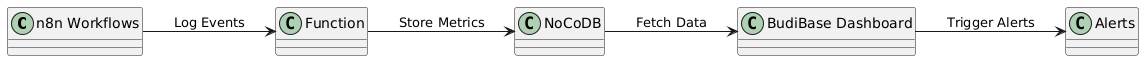
\includegraphics{figures/09-analytics-workflow}
    \caption{An analytics workflow example}
    \label{fig:analytics-workflow-example}
\end{figure}

\subsubsection{Step 3: Prepare for Scaling}
Adapt your automations to work for multiple clients:

\begin{itemize}
    \item Implement multi-tenancy in your NoCoDB database
    \item Create templates in BudiBase for quick client onboarding
    \item Develop a system for managing and updating multiple n8n workflows efficiently
\end{itemize}

\subsection{Common Challenges and Solutions}
\begin{itemize}
    \item Challenge: Maintaining performance as data volume grows
    \item Solution: Implement database indexing in NoCoDB. Use n8n's batch processing features for large datasets

    \item Challenge: Ensuring data segregation when scaling to multiple clients
    \item Solution: Implement strict access controls in NoCoDB. Use separate n8n workflows or add client identification steps in shared workflows
\end{itemize}

\subsection{Check-In and Reflection}
As you near the end of your 90-day journey, consider your progress on optimization and scaling:

\begin{itemize}
    \item How have you improved the performance of your automations?
    \item What insights have you gained from your analytics implementation?
    \item How prepared do you feel to scale your automations across multiple clients?
    \item Share a screenshot of your analytics dashboard in the Business Automators Discord community
\end{itemize}

\section{Weeks 11-12: Final Project and Evaluation}

\subsection{Objectives}
\begin{itemize}
    \item Complete a comprehensive automation project
    \item Evaluate the overall impact of your automation journey
    \item Prepare to showcase your work to potential clients
\end{itemize}

\subsection{Action Steps}

\subsubsection{Step 1: Final Automation Project}
Put all your skills together in a final, comprehensive project:

\begin{itemize}
    \item Choose a complex business process to automate fully
    \item Incorporate n8n, NoCoDB, and BudiBase in your solution
    \item Implement advanced features like error handling, scalability, and analytics
\end{itemize}

\subsubsection{Step 2: Comprehensive Evaluation}
Assess the impact of your 90-day automation journey:

\begin{itemize}
    \item Calculate total time saved across all your automation projects
    \item Evaluate improvement in task accuracy and consistency
    \item Gather feedback from team members or clients who have interacted with your automations
\end{itemize}

\subsubsection{Step 3: Prepare Your Showcase}
Create materials to demonstrate your new automation capabilities:

\begin{itemize}
    \item Develop a portfolio of your automation projects
    \item Create case studies highlighting the problems solved and benefits achieved
    \item Prepare a demo environment to show potential clients your automation skills in action
\end{itemize}

\subsection{Common Challenges and Solutions}
\begin{itemize}
    \item Challenge: Combining multiple tools and technologies in a single project
    \item Solution: Plan your architecture carefully. Use n8n as the central orchestrator, connecting NoCoDB for data storage and BudiBase for user interfaces

    \item Challenge: Quantifying the full impact of your automation efforts
    \item Solution: Use a combination of hard metrics (time saved, errors reduced) and soft metrics (client satisfaction, team feedback). Consider using a balanced scorecard approach
\end{itemize}

\subsection{Final Check-In and Reflection}
As you complete your 90-day automation journey, take time for a final reflection:

\begin{itemize}
    \item What has been your most significant achievement over the past 90 days?
    \item How has your approach to client projects changed with your new automation skills?
    \item What areas do you want to continue developing in the future?
    \item Share your final project and overall journey reflection in the Business Automators Discord community
\end{itemize}

\section{Conclusion: Your Automation Journey Continues}

Congratulations on completing this 90-day automation action plan! You've come a long way, from setting up your first basic automation to implementing complex, multi-tool solutions that can significantly impact your IT consulting practice.

Let's recap some key achievements:

\begin{itemize}
    \item Mastered key tools: n8n, NoCoDB, and BudiBase
    \item Completed at least 6 automation projects
    \item Integrated multiple systems and external APIs
    \item Developed skills in optimization, analytics, and scaling
    \item Created a portfolio to showcase your new capabilities
\end{itemize}

Remember, this is not the end, but rather the beginning of your journey as an automation-focused IT consultant. The field of automation is constantly evolving, and there will always be new tools, techniques, and challenges to explore.

To continue your growth:

\begin{itemize}
    \item Stay active in the Business Automators Discord community
    \item Regularly revisit and optimize your existing automations
    \item Keep learning about new features and integrations for n8n, NoCoDB, and BudiBase
    \item Explore additional tools and technologies that can complement your automation stack
    \item Share your knowledge by mentoring others or creating content about your automation experiences
\end{itemize}

As you move forward, remember that the true value of automation lies not just in the time and effort saved, but in the enhanced value you can provide to your clients. Use your new skills to deliver more strategic, impactful solutions that drive real business outcomes.

Thank you for embarking on this 90-day journey. Here's to your continued success as an automation-empowered IT consultant!

% TODO @qr: Generate a QR code linking to the Business Automators Discord community

\clearpage

\section{Addendum: Weekly Progress Tracker}

Use this weekly progress tracker to monitor your achievements, challenges, and learnings throughout your 90-day journey. Fill it out at the end of each week to maintain momentum and track your growth.

\begin{table}[h]
    \centering
    \begin{tabular}{|p{2cm}|p{3cm}|p{3cm}|p{3cm}|p{3cm}|}
        \hline
        \textbf{Week} & \textbf{Achievements} & \textbf{Challenges} & \textbf{Time Saved} & \textbf{Next Week's Goals} \\
        \hline
        1 &  &  &  &  \\
        \hline
        2 &  &  &  &  \\
        \hline
        3 &  &  &  &  \\
        \hline
        4 &  &  &  &  \\
        \hline
        5 &  &  &  &  \\
        \hline
        6 &  &  &  &  \\
        \hline
        7 &  &  &  &  \\
        \hline
        8 &  &  &  &  \\
        \hline
        9 &  &  &  &  \\
        \hline
        10 &  &  &  &  \\
        \hline
        11 &  &  &  &  \\
        \hline
        12 &  &  &  &  \\
        \hline
    \end{tabular}
    \caption{Weekly Progress Tracker}
    \label{tab:progress-tracker}
\end{table}

Remember to share your progress and insights regularly in the Business Automators Discord community. Your experiences can inspire others, and you may gain valuable advice from fellow automation enthusiasts.

Keep this tracker handy and update it diligently. It will not only help you stay on track during these 90 days but also serve as a valuable record of your automation journey that you can look back on in the future.

Good luck, and happy automating!